\documentclass[10pt, a4paper, twocolumn]{article}
\usepackage{algorithm}
\usepackage{algorithmic}
\usepackage{setspace}
\usepackage{graphicx}
\usepackage{subfigure}
\begin{document}

Hahhha

\begin{algorithm}
\caption{Calculate $y = x^n$}
\label{alg1}
\begin{algorithmic}
\REQUIRE $n \geq 0 \vee x \neq 0$
\ENSURE $y = x^n$
\STATE $y \leftarrow 1$
\IF{$n < 0$}
\STATE $X \leftarrow 1 / x$
\STATE $N \leftarrow -n$
\ELSE
\STATE $X \leftarrow x$
\STATE $N \leftarrow n$
\ENDIF
\WHILE{$N \neq 0$}
\IF{$N$ is even}
\STATE $X \leftarrow X \times X$
\STATE $N \leftarrow N / 2$
\ELSE[$N$ is odd]
\STATE $y \leftarrow y \times X$
\STATE $N \leftarrow N - 1$
\ENDIF
\ENDWHILE
\end{algorithmic}
\end{algorithm}
x\\

\begin{figure}
\centering
\subfigure{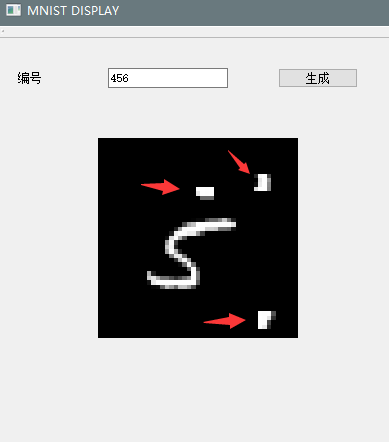
\includegraphics{mnist_display.png}}
\subfigure{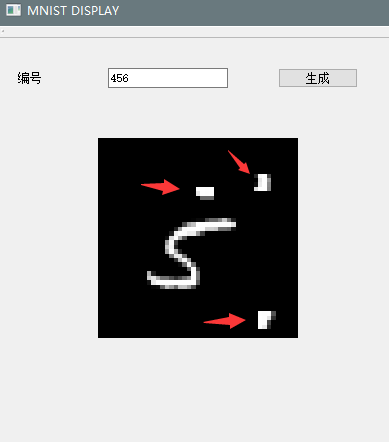
\includegraphics{mnist_display.png}}
\subfigure{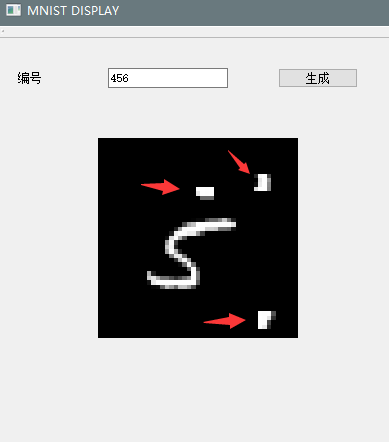
\includegraphics{mnist_display.png}}
\subfigure{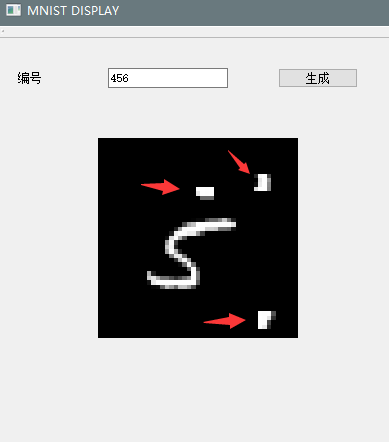
\includegraphics{mnist_display.png}}
\caption{ Dynamics of hysteretic neurons with different initial
noise amplitudes $A(0)$. (a) Dynamics of the proposed hysteretic
neuron with $A(0)=0.01$; (b) Dynamics of the proposed hysteretic
neuron with $A(0)=0.003$; (c) Dynamics of the neuron using the
previous hysteretic activation function with $A(0)=0.01$; (d)
Dynamics of the neuron using the previous hysteretic activation
function with $A(0)=0.003$.} \label{fig4}
\end{figure}



\end{document}
